\documentclass[12pt,letterpaper]{book}
\usepackage[utf8]{inputenc}
\usepackage[spanish]{babel}
\usepackage{latexsym,amsmath,amssymb,amsthm}
\usepackage{graphicx}
\usepackage{pifont}
\usepackage[pdftex=true,colorlinks=true,plainpages=false]{hyperref}
\hypersetup{urlcolor=blue}
\hypersetup{linkcolor=black}
\hypersetup{citecolor=black}
\usepackage{lastpage}
\usepackage{url}
\usepackage{anysize} 
\marginsize{2.5cm}{1.5cm}{1cm}{1.2cm}
\usepackage{fancyhdr}
\usepackage{anyfontsize}
\usepackage{tocbibind}
%%%% \slshape 

\pagestyle{fancy}
\lhead{\small \slshape \leftmark} \chead{} \rhead{\small \slshape \rightmark}
\lfoot{\url{http://scesi.fcyt.umss.edu.bo}} \cfoot{
\includegraphics[scale=0.25]{gnome/logo.png}} \rfoot{\thepage/\pageref{LastPage}}
\renewcommand{\headrulewidth}{0.4pt}
\renewcommand{\footrulewidth}{0.3pt}
\setlength{\headsep}{0.9\headsep}
\setlength{\footskip}{1.3\footskip}

%\title{Gnome}
%\author{Ubaldino Zurita}
%\date{\today}

\begin{document}
 \begin{titlepage}
	\thispagestyle{empty}
	\begin{center}
		\includegraphics[scale=0.7]{gnome/gnome-3.jpg} \\
		~\\
		\Large{\textsc{\bf Universidad Mayor De San Simón}}\\
		\large{\textsc{\bf Facultad De Ciencias y Tecnológica}}\\
		\large{\textsc{\bf Sistemas e Informática}}\\
		~\\
		\small{\bf \today}
	\end{center}
 	\vfill
	\begin{center}
		\Huge{\underline{\textsc{\bf Gnome}}}
	\end{center}
	\vfill
	\hrule
	\vspace{0.1cm}
	\noindent\small{\url{http://scesi.fcyt.umss.edu.bo} \hfill \url{http://www.memi.umss.edu.bo}}
	\hrule
	\vspace{0.1cm}
	\noindent\small{\hspace{1.35cm}
\includegraphics[scale=0.06]{gnome/scesi.png} \hfill 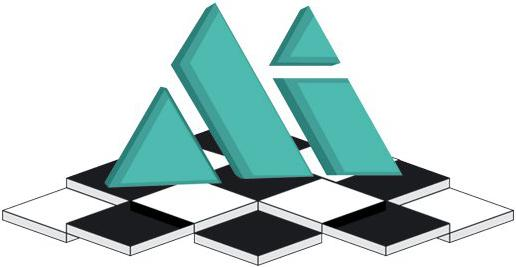
\includegraphics[scale=0.21]{gnome/memi.jpg}\hspace{0.43cm}}

\end{titlepage}

%\maketitle
\tableofcontents
%\setcounter{page}{1}
\part{INICIO DE SESIÓN}
\chapter{Pantalla de inicio de sesión}
\section{La pantalla de inicio de sesión incluye los siguientes elementos}
\begin{description}
\item[Solicitud de entrada] Escriba su nombre de usuario y contraseña para iniciar la sesión.
\item[Menú Idioma] Seleccione un idioma para la sesión.
\item [Menú Tipo de sesión] Seleccione el escritorio que se debe ejecutar durante la sesión. Si hay instalados otros escritorios, aparece
\item[Menú Idioma] Seleccione un idioma para la sesión.
\item [Menú Tipo de sesión] Seleccione el escritorio que se debe ejecutar durante la sesión. Si hay instalados otros escritorios, aparecerán en la lista.\\ pero en nuestro caso es {\bf Gnome 3.}
\item[Reiniciar] Reinicia el equipo.
\item[Apagar] Apaga el equipo.
\end{description}
\subsubsection{Inicio de sesión}
Una sesión es la entrada de un usuario a su cuenta en el sistema operativo instalado la cual tiene una pantalla de entrada que ofrece varias opciones relacionadas.\\
Por ejemplo, se puede seleccionar el idioma de la sesión, de modo que el texto de la interfaz aparezca en el idioma seleccionado.\\
Una vez que se autentican el nombre de usuario y la contraseña, se inicia el administrador de sesiones, el cual permite guardar determinados valores de configuración de cada sesión. También permite guardar el estado de la sesión más reciente y recuperarla la próxima vez que entre.\\
El administrador de sesiones permite guardar y restaurar los siguientes ajustes:
\begin{itemize}
\item[$\bullet$] Configuración de visualización y funcionamiento del escritorio, como fuentes, colores y configuración del ratón.
\item[$\bullet$] Aplicaciones que se están ejecutando, como un gestor de archivos o un programa de OpenOffice.org.
\end{itemize}
{\bf \underline{A tener en cuenta}}\\
No es posible guardar ni restaurar aplicaciones que no gestione el administrador de sesiones. Por ejemplo, si se inicia el editor vim en la línea de comandos de una ventana de terminal, el administrador de sesiones no puede restaurar la sesión de edición.

\section{Salida de sesión}
Cuando haya terminado de usar el equipo, puede salir de la sesión y dejar el sistema en ejecución, o bien reiniciar o apagar el equipo.\\
\subsection{Salida de la sesión o cambio de usuario}
\begin{enumerate}
\item Haga clic en Ordenador $=>$ Salir.
\item Seleccione una de las siguientes opciones:
\begin{description}
\item[Salir de la sesión] Se sale de la sesión en curso y se vuelve a la pantalla de entrada a la sesión.
\item[Cambiar de usuario] Se suspende la sesión y se permite que otro usuario entre y utilice el equipo.
\end{description}
\end{enumerate}
\subsection{Reinicio o cierre del equipo}
\begin{enumerate}
\item Haga clic en Ordenador $=>$ Apagar.
\item Seleccione una de las siguientes opciones:
\begin{description}
\item[Apagar] Se cierra la sesión actual y se apaga el equipo.
\item[Reiniciar] Se cierra la sesión actual y se reinicia el equipo.
\item[Reposo] El equipo adopta un estado temporal de ahorro de energía. Se mantiene el estado de la sesión, incluidas todas las aplicaciones en ejecución y todos los documentos abiertos.
\item[Hibernar] Se suspende la sesión y no se emplea electricidad hasta que se reinicia el equipo. Se mantiene el estado de la sesión, incluidas todas las aplicaciones en ejecución y todos los documentos abiertos.
\end{description}
\end{enumerate}
%------------------------------------------------------
\part{GNOME}
\chapter{Contenido y Uso de Gnome Shell}
\begin{center}
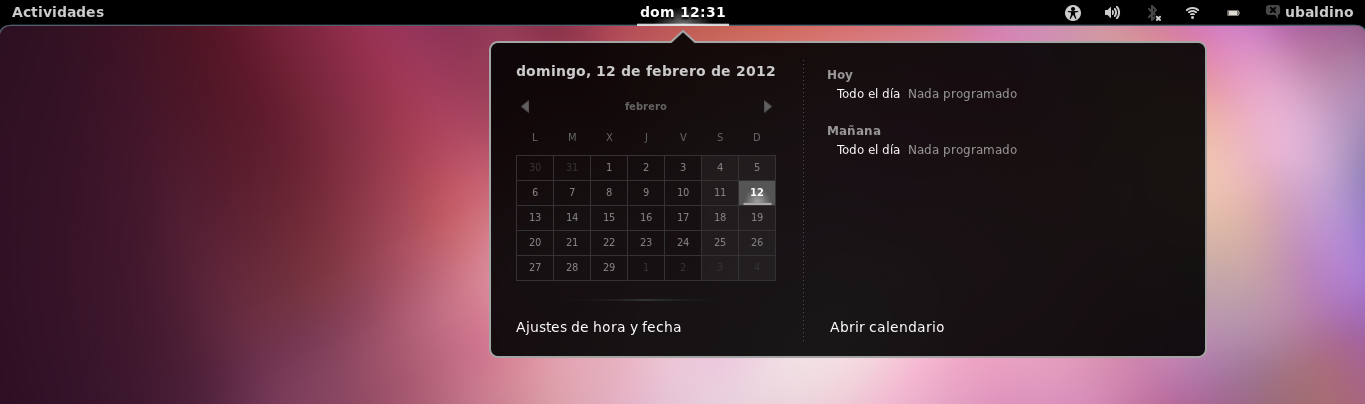
\includegraphics[scale=0.448]{gnome/barra.png}
\end{center}
Gnome es uno de los tantos escritorios que existen para las distribuciones basadas en linux.
En este caso UBUNTU 11.10 utiliza el escritorio o interfaz gráfica Gnome 3, y como es de esperar de un escritorio, los componentes principales del escritorio Gnome son:
\begin{itemize}
\item[-] Iconos que enlazan a archivos, carpetas o programas (accesos directos).
\item[-] Gnome Shell que es la barra de tareas y lanzador de aplicaciones. y tiene un gestor de ventanas con soporte OpenGL.
\begin{description}
\item[Gnome Shell] tiene un panel único en la parte superior, que contiene:
\begin{itemize}
 \item menú de usuario. 
 \item un botón “actividades”. 
 \item aplicaciones en ejecución.
 \item reloj.
 \item área de accesibilidad.
 \item control de volumen.
 \item información de la red.
 \item estado de la batería en el caso de un portátil.
\end{itemize}
En el arranque del sistema aparece dicho panel y el fondo de escritorio.
\end{description}
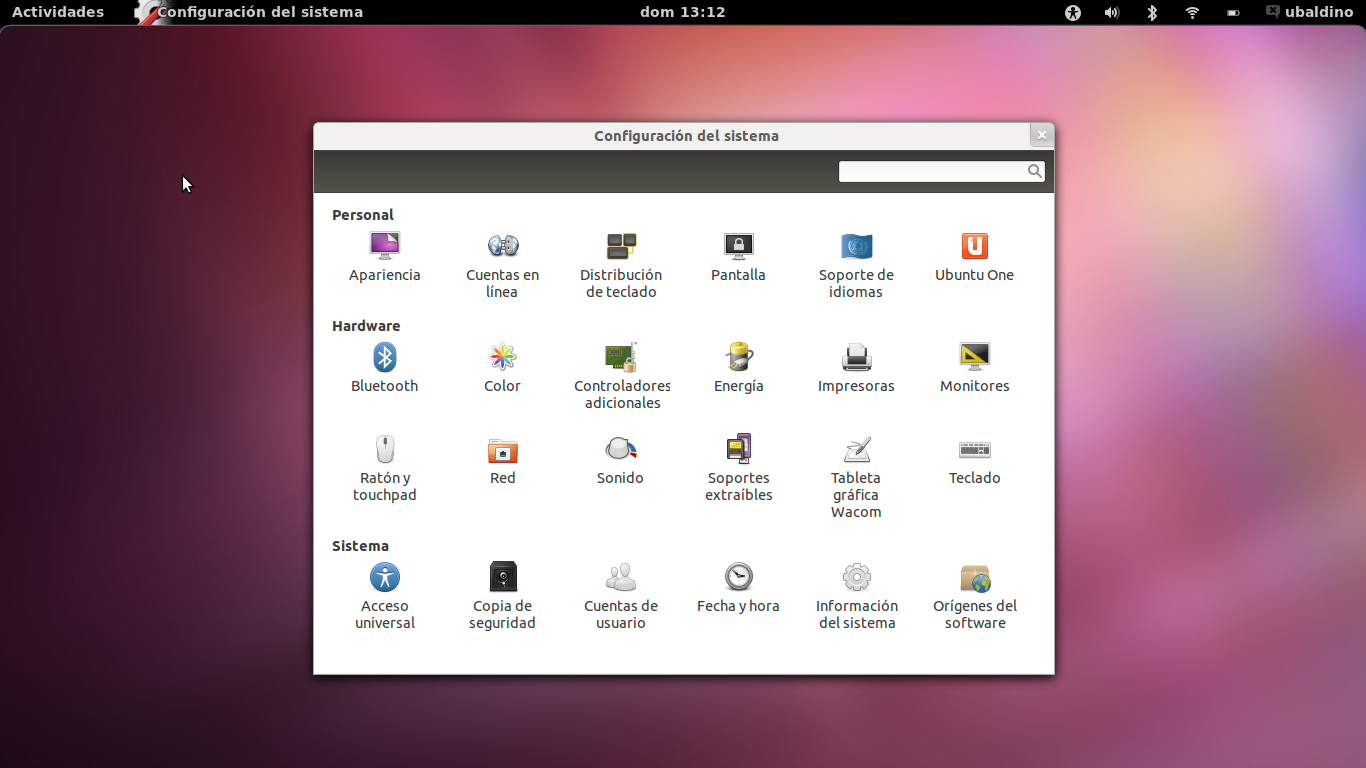
\includegraphics[scale=0.35]{gnome/Pantallazo3.png}\\ 
Al pulsar sobre “actividades” o acercar el ratón con rapidez a la esquina superior izquierda, se despliegan varios elementos nuevos:
\begin{itemize}
\item A la izquierda, un panel lanzador de aplicaciones,
\item Bajo el panel superior, un menú de dos opciones, “ventanas” y “aplicaciones”.
\item A la derecha, otro panel con una vista previa de las ventanas activas que actúa como selector de escritorios y por encima de éste, una caja de búsqueda.
\end{itemize}
Si tienes ya algún programa en ejecución, que por defecto se lanza a pantalla completa, la ventana o ventanas activas que su reducen su tamaño mostrando una leyenda informativa en la parte inferior de cada ventana. Cada acción que comporte cambios de tamaño o posición, vendrá acompañada de una elegante animación y otros efectos visuales.\\
El botón gráfico windows (ventanas), restaura la vista previa de aquellas que estén activas si las has perdido de vista por ejecutar cualquier otra acción.\\
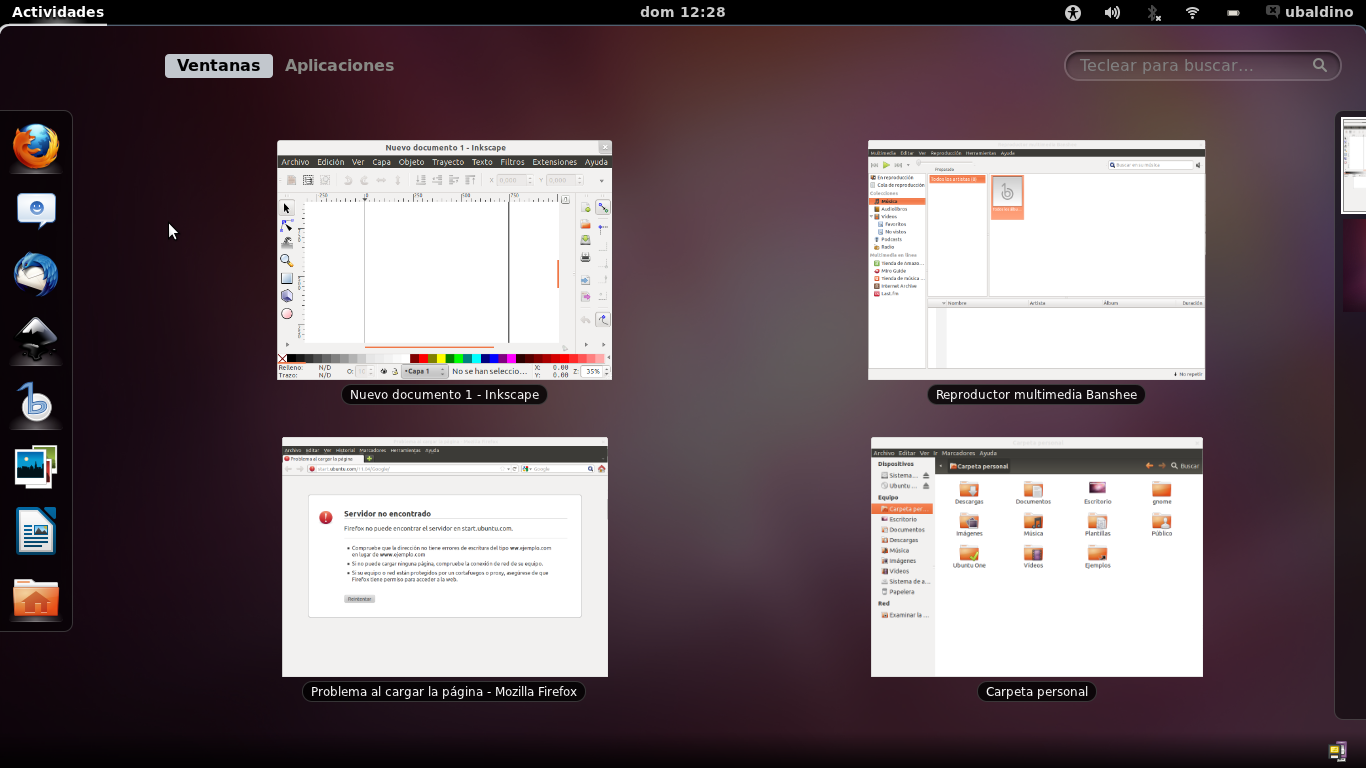
\includegraphics[scale=0.35]{gnome/Pantallazo4.png}\\ 

El botón aplications (aplicaciones), da paso a la representación mediante iconos de los programas instalados en la máquina.\\

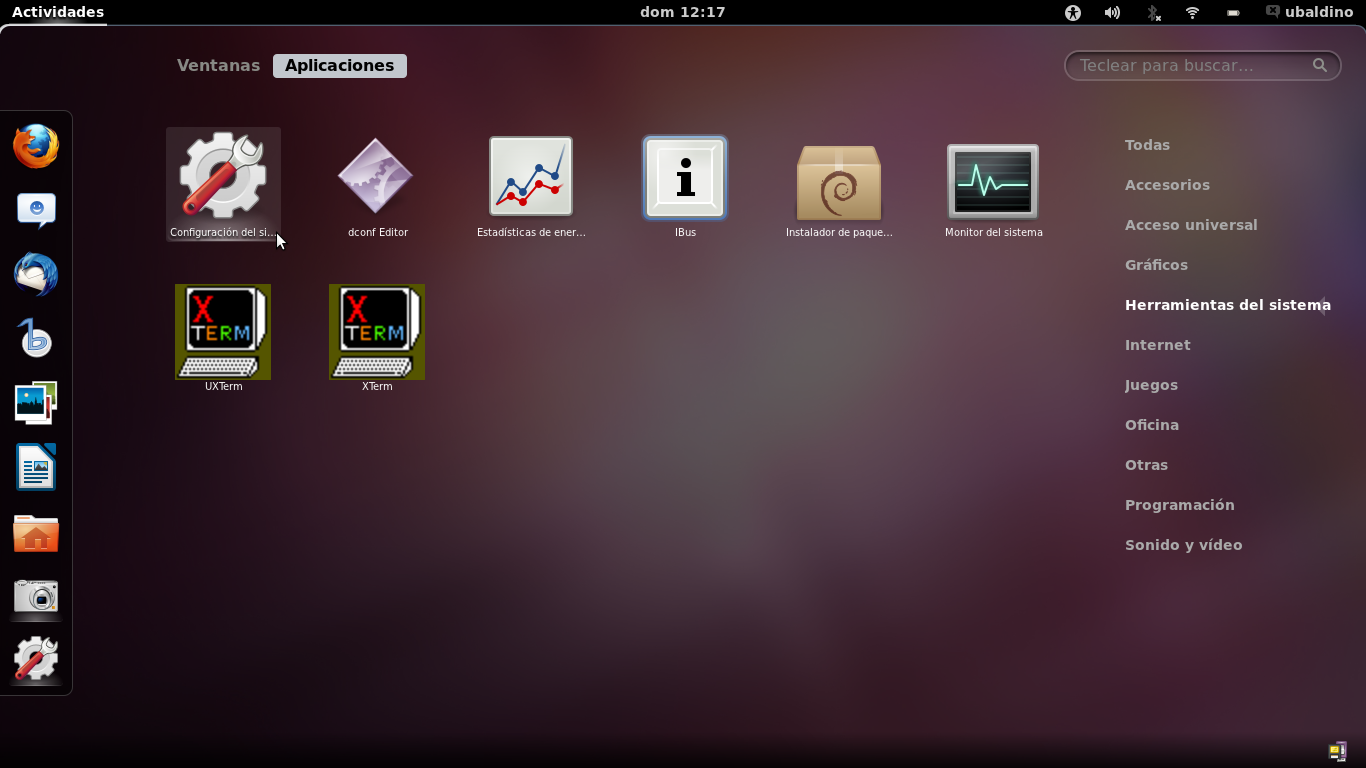
\includegraphics[scale=0.35]{gnome/Pantallazo5.png} \\
\underline{\bf Nota:} Note que cuando estamos en la presentación de los programas instalados en la maquina. El panel de la derecha porta un sistema de filtrado, clasificando los programas según las funcionalidades.\\
\newpage
La caja de búsqueda es lo novedoso de gnome 3. Escribiendo las primeras letras de una aplicación, aparecerá de forma inmediata el icono correspondiente al programa y puedes lanzar la aplicación desde ahí. Y en la parte inferior de la pantalla muestra dos botones gráficos, que permiten extender la búsqueda en Wikipedia y Google.\\ 

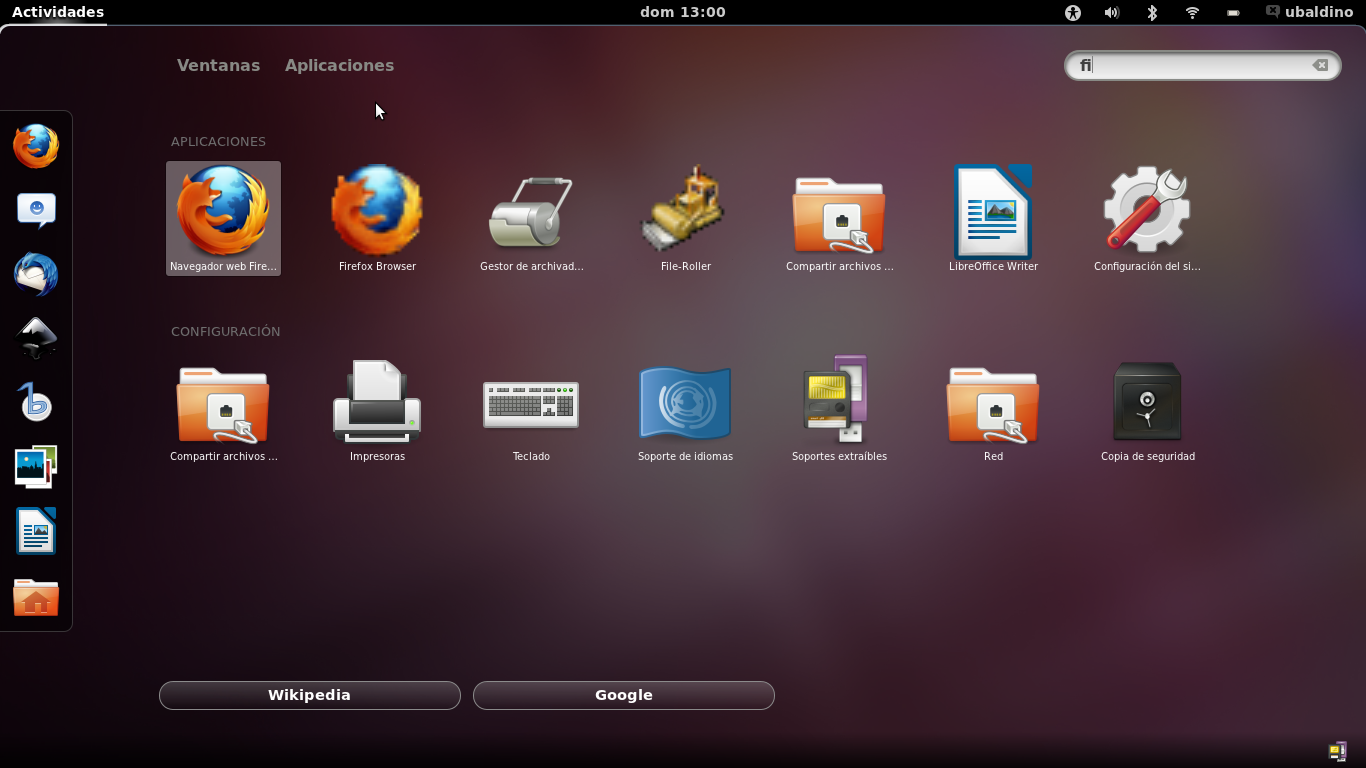
\includegraphics[scale=0.35]{gnome/Pantallazo6.png}\\ 
\newpage
Por último, terminando nuestro recorrido en Gnome Shell, en la parte inferior derecha de la pantalla veremos el área de notificaciones y bandeja de mensajes, desde donde puedes contestar con el programa de mensajería instantánea.\\
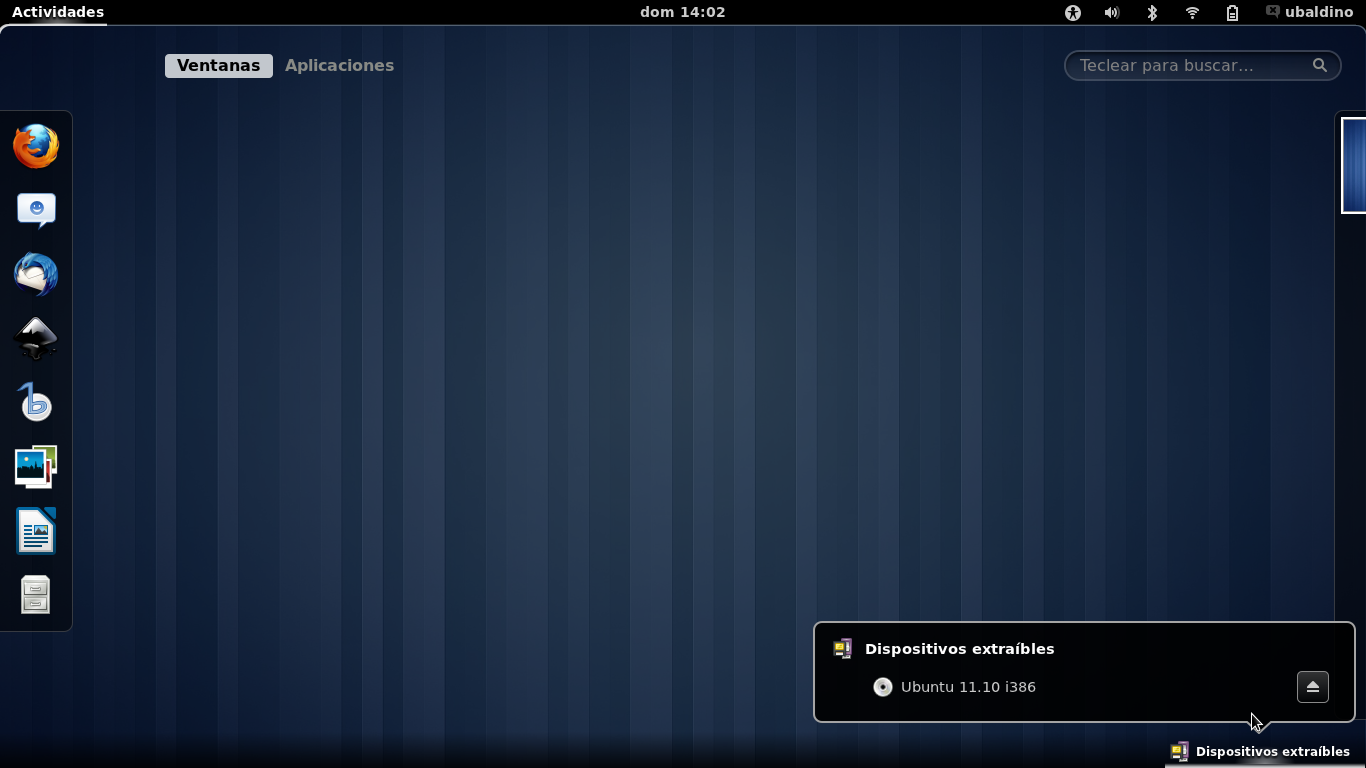
\includegraphics[scale=0.35]{gnome/Pantallazo7.png} 
\end{itemize}
\chapter{Personalización}
Se puede cambiar el aspecto y el comportamiento del escritorio Gnome para que se adapte a preferencias y necesidades personales. Algunos de los ajustes que puede querer cambiar incluyen:
\begin{itemize}
\item Configuración del teclado y el ratón.
\item Modificación de preferencias del teclado.
\item Configuración del ratón.
\item Fondo del escritorio.
\item Protector de pantalla.
\item Contraseña.
\item Sonidos.
\end{itemize}
Estos ajustes, entre otros, se pueden cambiar en el Centro de control.
\section{Herramientas del sistema}
Para acceder al centro de control, haga clic en {\bf actividades $=>$ aplicaciones $=>$ panel derecho herramientas del sistema $=>$ Configuración del sistema}. Este se encuentra dividido en las tres categorías siguientes:
\begin{description}
\item[Personal] Acceda aquí para cambiar los valores de configuración del fondo de escritorio. Puede modificar los temas, agregar o quitar idiomas y poder configurar la distribución del teclado que desee utilizar.
\item[Hardware] Permite configurar componentes de hardware, como tarjetas gráficas, monitores, impresoras o para configurar los accesos directos y los atajos de teclado, así como instalar dispositivos de red y configurar la conexión de red.
\item[Sistema] Permite configurar valores del sistema como la fecha y la hora y cambiar
la contraseña de entrada o los valores de accesibilidad.
También podrá cambiar direcciones de los servidores de software y obtener información de su sistema 
\end{description}
\begin{center}
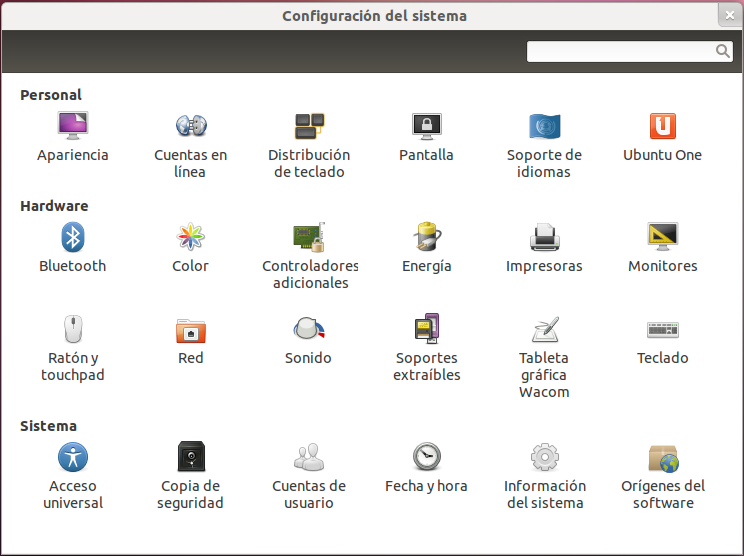
\includegraphics[scale=0.6]{gnome/Pantallazo31.png}\\
\end{center}
Para cambiar algunos de los valores globales del sistema, Gnome solicitará
la contraseña del usuario Administrador. Es el caso principalmente de los
valores del administrador, que incluyen la mayor parte de los valores de configuración
del hardware, la interfaz gráfica del usuario, el acceso a Internet, la seguridad, la
administración de usuarios o la instalación de software, así como las actualizaciones y
la información del sistema.
%--------------------------------------------------------------
\section{Personal}
En esta sección veremos ejemplos sobre cómo configurar algunos aspectos personales del escritorio Gnome, como la accesibilidad y la configuracion de la hora y fecha o la compatibilidad con la tecnología de asistencia, así como sobre la forma de cambiar la contraseña o gestionar anillos de claves virtuales.
	\subsection{Apariencia}
	\begin{center}
	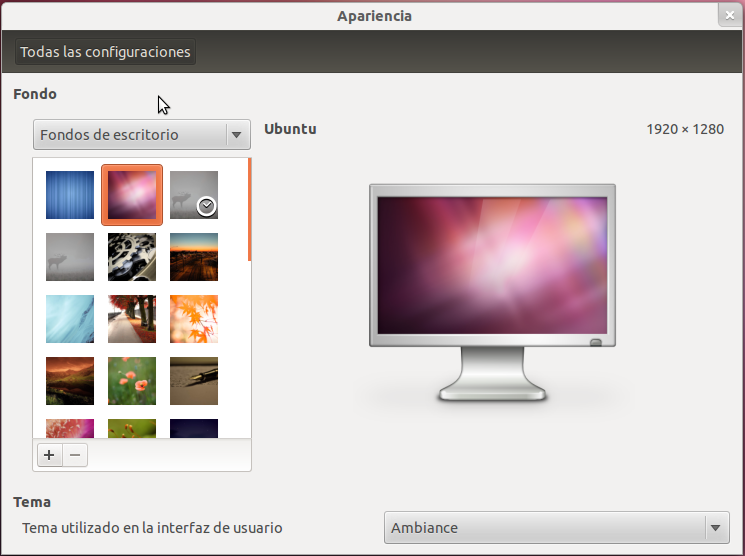
\includegraphics[scale=0.6]{gnome/apariencia.png}
	\end{center}	
		\begin{itemize}
			\item {\large \bf Cambiar el fondo del escritorio}
				
					Puede cambiar la imagen usada en el fondo del escritorio o establecer un color simple o degradado.\\

Seleccione una imagen o un color. La configuración se aplicará inmediatamente.\\

Existen tres opciones en la lista desplegable en la izquierda.
\begin{itemize}
\item Seleccione Fondos de escritorio para usar una de las muchas imágenes de fondo profesionales con las que se distribuye GNOME. Algunos fondos de escritorio son parcialmente transparentes y permiten mostrar un color de fondo a través de ellos. Para esos fondos de escritorio, existirá un botón de selección de color en la esquina inferior derecha.
\item Seleccione la carpeta Imágenes para usar una de sus propias fotografías de su carpeta Imágenes. La mayoría de los gestores de fotos almacenan las fotos aquí.
\item Seleccione Color y gradientes para ajustar un color plano o un gradiente lineal. Los botones selectores de color aparecerán en la esquina inferior derecha.
\end{itemize}
También puede buscar una imagen en su equipo pulsando el botón +. Cualquier imagen que añada de esta manera se mostrará en la carpeta de Imágenes.\\
Puede quitarla de la lista seleccionándola y pulsando el botón -. Quitar una imagen de la lista no eliminará el archivo original.

			\item {\large \bf Cambiar el tema del escritorio}
			Un tema es un grupo de ajustes que especifican el aspecto visual de una parte del escritorio. Los usuarios pueden seleccionar temas para cambiar el aspecto del escritorio.\\

Seleccione una tema de su preferencia. La configuración se aplicará inmediatamente.\\
Un tema contiene ajustes que afectan a distintas partes del escritorio, como se describe
a continuación:
\begin{description}
\item[Controles] El ajuste de controles de los temas determina el aspecto visual de las ventanas, paneles y applets. También determina el aspecto visual de los elementos de la interfaz compatible con GNOME que se muestran en las ventanas, paneles y applets (como menús, iconos y botones). Algunas de las opciones de ajuste de los controles disponibles están diseñadas para necesidades de accesibilidad especiales.
\item[Marco de las ventanas] El ajuste de los marcos de las ventanas de un tema determina únicamente el aspecto de los marcos que rodean las ventanas.
\item[Icono] El ajuste de los iconos de un tema determina el aspecto de los iconos en los paneles y el fondo del escritorio.
\end{description}
		\end{itemize}
	\subsection{Distribución del teclado}
	Los teclados vienen en cientos de distribuciones diferentes para distintos idiomas. Incluso para un solo idioma pueden existir muchas distribuciones de teclado, como la distribución Dvorak para el inglés. Puede hacer que su teclado se comporte como un teclado con una distribución diferente, independientemente de que letras y símbolos tenga escritos en las teclas. Esto es útil si tiene que usar varios idiomas a menudo.\\

Abra distribución del teclado\\

Nos encontraremos con cuatro pestañas que veremos a continuación:
\begin{itemize}
	\item {\large \bf Idioma}\\
	En esta pestaña puede anadir varios idiomas para que el teclado se comunique con nuestro sistema\\
    Pulsando el botón +, añade un idioma\\
    Pulsando el boton -, elimina un idioma
\begin{center}
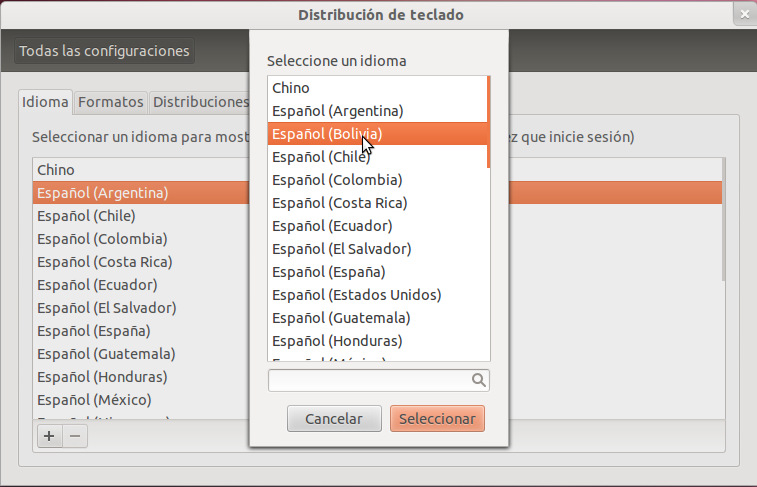
\includegraphics[scale=0.6]{gnome/idioma1.png} 
\end{center}
	\item {\large \bf Formatos}\\
		Esta pestaña te mostrara la forma de mostrar información que sera adecuada a tu zona para la cual elegimos.
\begin{center}
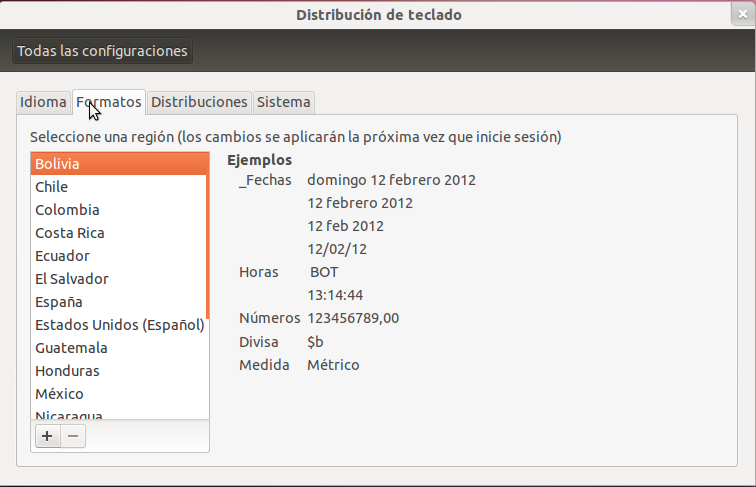
\includegraphics[scale=0.6]{gnome/formato.png} 
\end{center}
Podemos añadir como también eliminar regiones.\\ 
		Cuando cambia su región para los formatos, sólo lo cambia para su cuenta después de iniciar la sesión.
	\item {\large \bf Distribuciones}\\
	Los teclados vienen en cientos de distribuciones diferentes para distintos idiomas. Incluso para un solo idioma pueden existir muchas distribuciones de teclado, como la distribución Dvorak para el inglés. Puede hacer que su teclado se comporte como un teclado con una distribución diferente, independientemente de que letras y símbolos tenga escritos en las teclas. Esto es útil si tiene que usar varios idiomas a menudo.
Pulse en su nombre en la barra superior y seleccione Configuración del sistema.\\

Seleccione la pestaña Distribuciones.\\
Pulse el botón +, seleccione una distribución y pulse Añadir. Puede añadir hasta cuatro distribuciones.\\
Puede tener una vista previa de una imagen o cualquier distribución seleccionando en la lista y pulsando la imagen de teclado, o pulsando Vista previa en la ventana emergente cuando añade una distribución.\\
Cuando se añaden varias distribuciones, puede cambiar entre ellas utilizando el icono de distribución de teclado en la barra superior. La barra superior mostrará una cadena corta de identificación de la distribución actual, tal como es para la distribución estándar de español. Pulse en el indicador de la distribución y seleccione la que quiera usar en el menú.\\
Cuando se usan varias distribuciones, se puede elegir entre tener todas las ventanas con la misma distribución o asignar una distribución diferente a cada ventana. Este último resulta interesante, por ejemplo, si esta escribiendo un articulo en otro idioma en una ventana del procesador de textos. Cada ventana recordara su selección de teclado conforme vaya pasando de una ventana a otra.\\

De manera predeterminada, las nuevas ventanas usaran la distribución de teclado predeterminada. En su lugar, puede elegir que usen la distribución de la ventana que estuviera usando antes. La distribución predeterminada es la situada al principio de la lista. Use los botones $\uparrow$ y $\downarrow$ para subir o bajar las distribuciones dentro de la lista.
	\item {\large \bf Sistema}\\
	Simplemente muestra los ajustes del sistema.	
	\begin{center}
		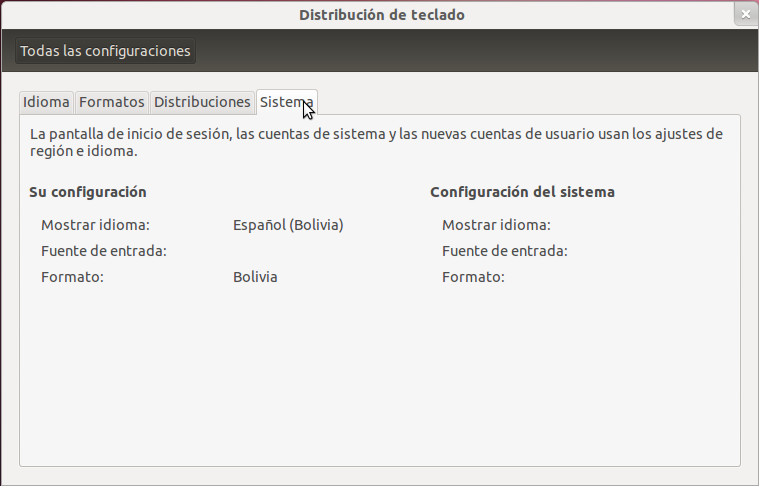
\includegraphics[scale=0.6]{gnome/sistema1.png} 
    \end{center}
\end{itemize}
\subsection{Pantalla}
Puede cambiar el brillo de su pantalla para ahorrar energía o hacerla más legible en condiciones de mucha luz ambiental. También puede hacer que la pantalla se atenúe automáticamente cuando se consume batería o apagarla automáticamente cuando no se use la pantalla.\\

Establecer el brillo\\

Abra Pantalla.
Mueva el deslizador de Brillo para obtener un valor confortable.\\

Muchas portátiles tienen teclados con teclas especiales para ajustar el brillo. Éstas tienen una imagen que parece un sol y están ubicadas en las teclas de función en la parte superior. Mantenga pulsada la tecla Fn para usar estas teclas.\\

Seleccione oscurecer para ahorrar energía, la pantalla se reducirá  automáticamente cuando esté usando la batería.\\
La luz de fondo de su pantalla puede consumir mucha energía y reducir significativamente el tiempo que durará la batería hasta que tenga que volver a cargarla.\\
La pantalla se apagará automáticamente cuando lleve un tiempo sin usarla.\\
Esto solo afecta a la pantalla, y no apaga su equipo. Puede ajustar el tiempo que tiene que estar inactivo en la lista desplegable Apagar después de:
\begin{center}
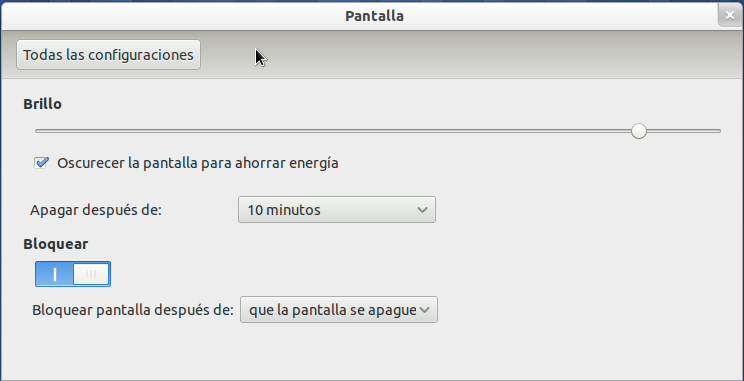
\includegraphics[scale=0.6]{gnome/pantallaa1.png} 
\end{center}
\subsection{Soporte de idiomas}
En esta sección aparecen los idiomas de soporte para las ventanas en orden por países por defecto esta primero España, pero puedes cambiar al país de tu preferencia con tan solo arrastrándolo hasta la posición que prefieras.
\begin{center}
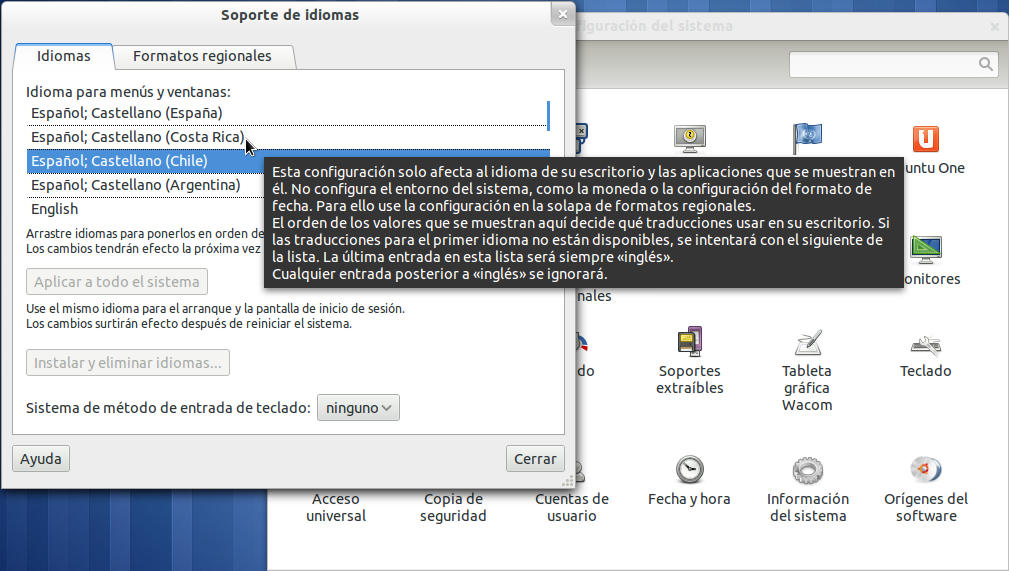
\includegraphics[scale=0.6]{gnome/idiomas2.png} 
\end{center}
En formatos regionales simplemente eliges el idioma y conjuntamente a la región de tu preferencia.
\begin{center}
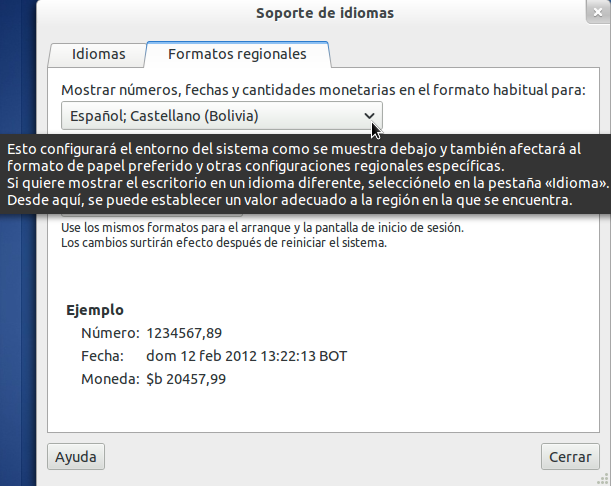
\includegraphics[scale=0.6]{gnome/idiomas3.png} 
\end{center}
%---------------------
\section{Hardware}
En esta sección veremos las configuraciones del hardware del escritorio Gnome, como las preferencias del teclado y del ratón, la gestión de unidades y medios extraíbles o la resolución de la pantalla.
\subsection{Modificación de preferencias del teclado}
Para modificar algunos valores de configuración, como las preferencias de repetición
automática o las sesiones de descanso de escritura, haga clic en Ordenador $>$ Centro
de control $>$ Hardware $>$ Teclado
\begin{enumerate}
\item En la ficha Teclado, puede definir algunas preferencias del teclado de carácter general, como habilitar la repetición con opciones de retardo y velocidad individuales, o habilitar e inhabilitar el parpadeo del cursor y definir la velocidad. Para obtener más información sobre cada una de las opciones, haga clic en Ayuda.
\item Para seleccionar el modelo del teclado, haga clic en la pestaña Distribuciones, haga clic en el botón Examinar y seleccione el modelo de la lista.
\item Para añadir una nueva distribución de idioma, haga clic en Añadir y elija una distribución de la lista. Puede seleccionar distintas distribuciones para ajustarlas a configuraciones regionales diferentes. Defina una distribución con el valor Por defecto.
\item En la pestaña Descanso de escritura puede definir las preferencias correspondientes. Para obtener más información sobre cada una de las opciones, haga clic
en Ayuda.
\item Cuando haya definido todas las opciones según sus preferencias, haga clic en Cerrar.
\end{enumerate}
\subsection{Ratón y Touchpad}
Entrando en la parte de Ratón y touchpad. \\
Seleccionando la pestaña Ratón, veras las siguientes opciones.\\
\begin{itemize}
\item{\large \bf Ratón}\\
\begin{itemize}
\item{\bf General}\\
Puede intercambiar el comportamiento de los botones izquierdo y derecho de su ratón o touchpad para poder estar más cómodo.\\
Seleccione Zurdo.
Este ajuste afectará tanto a su ratón como a su touchpad, así como a cualquier otro dispositivo apuntador.\\

Al activar la opción de mostrar la posición del puntero al pulsar la tecla control.\\
Pulsando Ctrl se visualizará una animación que aparecerá brevemente en la posición del puntero.
\item{\bf Velocidad del puntero}\\
Si el puntero se mueve demasiado deprisa o despacio cuando mueve el ratón, puede ajustar la sensibilidad del puntero y la aceleración para estos dispositivos.\\

Ajuste los deslizadores de Aceleración y Sensibilidad hasta que el movimiento del puntero le sea cómodo.
\item{\bf Arrastrar y soltar}\\
Cuando se pulsa sobre algo, no es raro que su mano se mueva un poco durante el tiempo que pasa entre que pulsa el botón y lo suelta. Por esa razón, el proceso de arrastrar solo empieza si se mueve el puntero pasado un cierto umbral, para que no empiece a arrastrar accidentalmente cada vez que pulse sobre algo.\\

En Arrastrar y soltar, ajuste el deslizador del Umbral a un valor que le resulte cómodo. Pruebe a mover la ventana de opciones arrastrando la barra de título para probar el valor actual.\\

Este ajuste afectará tanto a su ratón como a su touchpad, así como a cualquier otro dispositivo apuntador.
\item{\bf Tiempo de espera de la pulsación doble}\\
La doble pulsación solo sucede cuando pulsa el botón del ratón dos veces lo bastante rápido. Si se tarda mucho en pulsar la segunda vez, obtendrá dos pulsaciones separadas, no una doble pulsación. Si tiene dificultados en pulsar el ratón tan deprisa debería incrementar el tiempo de espera.\\

En Tiempo de espera de la pulsación doble, ajuste el deslizador Tiempo de espera a un valor que considere confortable. Use la cara sonriente junto al deslizador para probar su configuración. Una pulsación simple lo hará sonreír. Una pulsación doble lo hará sonreír de oreja a oreja.\\

Este ajuste afectará tanto a su ratón como a su touchpad, así como a cualquier otro dispositivo apuntador.
\end{itemize}
\begin{center}
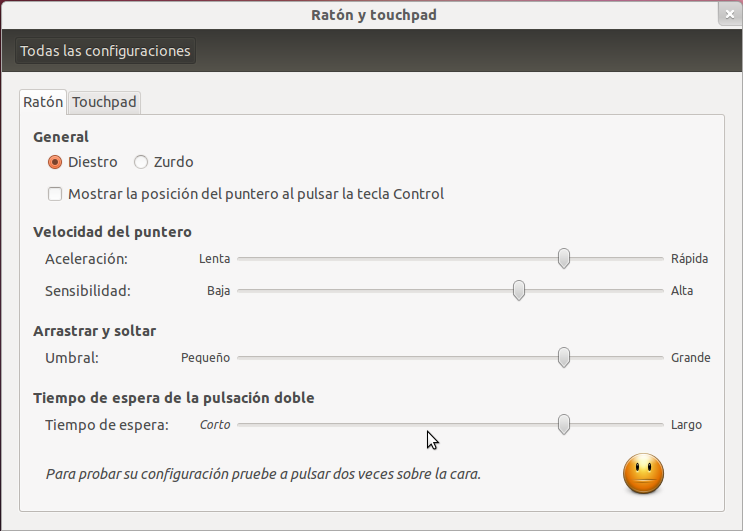
\includegraphics[scale=0.6]{gnome/raton.png} 
\end{center}
\item{\large \bf Touchpad}\\
Puedes pulsar, hacer dobles pulsaciones, arrastrar y desplazarse usando solo el touchpad, sin usar botones físicos aparte.\\
Solo estará disponible si su equipo tiene uno.
	\begin{center}
\includegraphics[scale=0.6]{gnome/touchpap.png}
\end{center} 
	\begin{itemize}
\item{\bf General}\\
Puedes activar o desactivar el touchpad cuando estas escribiendo o el acto de golpear y arrastrar con los dedos en el touchpad.\\ 

Para pulsar, pulsar dos veces y arrastrar con su touchpad seleccione Activar\\ pulsaciones del ratón con el touchpad.\\

Para pulsar toque el touchpad.\\
Para una doble pulsación, toque dos veces.\\
Para arrastrar un elemento, toque dos veces pero no levante su dedo después del segundo toque. Arrastre el elemento a donde quiera y después levante su dedo para soltarlo.\\
Si su touchpad es multitáctil, pulse con el botón derecho del ratón usando dos dedos a la vez. De lo contrario necesitará usar los botones del hardware para pulsar con el botón derecho del ratón. Para ver un método de pulsación derecha del ratón sin usar el segundo botón del ratón consulte la Simular una pulsación derecha del ratón.
\item{\bf Desplazamiento}\\
Si su touchpad soporta multi-toques puede elegir desplazamientos usando su touchpad, bien usando los bordes del touchpad o bien usando dos dedos.\\
\begin{itemize}
\item Seleccione Desplazamiento en el borde en Desplazamiento para hacer desplazamientos usando el borde de su touchpad.\\ Cuando está seleccionado, al arrastrar su dedo arriba y abajo por el lateral derecho de su touchpad se desplazará verticalmente.\\ Si además selecciona Activar desplazamiento horizontal, al arrastrar su dedo a izquierda y derecha por el borde inferior del touchpad se desplazará horizontalmente.

\item Seleccione Desplazamiento con dos dedos en Desplazamiento para desplazarse con dos dedos.\\
Cuando está seleccionado, el acto de golpear y arrastrar con un solo dedo funcionará como siempre, pero si arrastra dos dedos por cualquier zona del touchpad, hará un desplazamiento.\\ Si además selecciona Activar desplazamiento horizontal, podrá mover sus dedos a izquierda y derecha para desplazarse horizontalmente. Asegúrese de dejar un poco de espacio entre sus dedos. Si sus dedos están demasiado juntos, el touchpad podría creer que se trata de un único dedo grande.
\end{itemize}
\item{\bf Velocidad del puntero}\\
Si el puntero se mueve demasiado deprisa o despacio cuando usa el touchpad, puede ajustar la sensibilidad del puntero y la aceleración para este dispositivo.\\

Ajuste los deslizadores de Aceleración y Sensibilidad hasta que el movimiento del puntero le sea cómodo.\\

La sensibilidad es la velocidad inicial del puntero al mover su ratón.\\
Cuanto más mueva el ratón, más rápidamente se mueve el puntero con relación a su movimiento. Esto le ayuda a mover el puntero por la pantalla sin levantar la mano, mientras que le permite apuntar y pulsar de manera precisa. La aceleración controla este comportamiento.
\end{itemize}
\end{itemize}
\subsection{Red}
Entrando en la configuración de la red, encontraras dos opciones o tres si tienes adaptador de conexión inalámbrica.
\begin{itemize}
\item{\bf Cableada}\\
Para configurar la mayoría de las conexiones a redes cableadas, todo lo que necesita es conectar un cable de red. El icono de red en la barra superior dará vueltas o parpadeará durante varios segundos y después cambiara al icono de un zócalo cuando esté conectado.\\
Si esto no ocurriera, deberá asegurarse primero de que su cable de red está conectado.\\

Puede habilitar o deshabilitar la conexión de red presionando el botón de activar/desativar.
\item{\bf Inalámbrica}\\
Si tiene un equipo con una tarjeta inalámbrica que funcione puede conectarse a una red inalámbrica cercana para obtener acceso a Internet, ver archivos compartidos en la red y demás.\\

Puedes encender o apagar.\\
Activar el modo avión.\\
Configurar la red inalámbrica.\\

%%Pulse el icono de red en la barra superior y 
Para conectarse a una red pulse en el nombre de la red a la que quiere conectarse.\\
Si el nombre de la red no está en la lista, pruebe a pulsar Más para ver si la red está más abajo en la lista. Si sigue sin verla, puede que esté fuera del área de cobertura o puede que la red esté oculta.\\
Si la red está protegida por una contraseña (clave de cifrado), introduzca la contraseña cuando se le pida y pulse Conectar.\\
Si no conoce la clave, puede que esté escrita en la parte inferior del enrutador inalámbrico o de la estación base, en el manual de instrucciones, o puede tener que preguntar a la persona que administra la red inalámbrica.\\
El icono de red cambiará su apariencia según el equipo intente conectarse a la red.\\
Si la conexión se realiza correctamente, el icono cambiará a un punto con varias barras por encima. Más barras indican una conexión más fuerte a la red. Si no hay muchas barras, las conexión es débil y puede no ser posible.\\

Si la conexión no tiene éxito, se le puede preguntar su contraseña otra vez, o simplemente puede decirle que la conexión se ha desconectado. Hay varias razones que pueden hacer que esto pase; puede haber introducido mal la contraseña, la señal inalámbrica es muy débil o la tarjeta inalámbrica de su equipo tiene un problema, por ejemplo. Consulte el solucionador de problemas de red inalámbrica para obtener más ayuda.\\

Una conexión más fuerte a una red inalámbrica no significa necesariamente que vaya a tener una conexión a Internet más rápida, o que vaya a tener una velocidad de descarga mayor. La conexión inalámbrica conecta su equipo al dispositivo que proporciona la conexión a Internet (como un enrutador o un módem), pero las dos conexiones son diferentes, y por lo tanto tiene velocidades distintas.\\

{\large \bf hotspot}\\
Puede usar su equipo como un hotspot inalámbrico. Esto permite a otros dispositivos conectarse a su equipo sin necesidad de una red aparte, y permite a su equipo compartir una conexión a Internet configurada en otra interfaz, como una red cableada o una red de banda ancha móvil.\\

Pulse el botón Usar como hotspot.\\
Si ya está conectado a una red inalámbrica, se le preguntará si quiere desconectarse de esa red.\\
Un adaptador inalámbrico sólo puede conectarse o crear una única red al mismo tiempo.\\
Pulse Crear hotspot para confirmar.\\

Se generan automáticamente un nombre de red (SSID) y una clave de seguridad. El nombre de red estará basado en el nombre de su equipo. Otros dispositivos necesitarán esta información para conectarse al hotspot que acaba de crear.
\end{itemize}
\subsection{Sonido}
\begin{itemize}
\item{\bf Efectos de sonido}\\
\item{\bf Hardware}\\
\item{\bf Entrada}\\
\item{\bf Salida}\\
\item{\bf Aplicaciones}\\
\end{itemize}
\subsection{Configuración de unidades y medios extraíbles}
Se pueden utilizar una gran variedad de unidades y soportes extraíbles, incluidos dispositivos de almacenamiento, cámaras y escáneres, entre otros. La configuración de muchos de estos dispositivos se establece automáticamente durante la instalación. Para cambiar la configuración de una unidad o de otro dispositivo extraíble, haga clic en Ordenador $>$ Centro de control $>$ Hardware $>$ Unidades y soportes extraíbles.
Algunos de los ajustes de configuración posibles incluyen:
\begin{itemize}
\item Qué ocurre cuando se introduce un CD vacío en la unidad de CD
\item Qué ocurre cuando se introduce un CD de audio en la unidad
\item Si las imágenes se importan automáticamente desde una cámara digital cuando se conecta al equipo
\item Si los dispositivos de almacenamiento extraíbles se montan cuando se conectan al equipo
\item Si los PDA se sincronizan automáticamente cuando se conectan al equipo
\end{itemize}
En general, no es preciso cambiar los ajustes que ya estén configurados a menos que quiera modificar el comportamiento del equipo cuando se conecte un dispositivo o en caso de que quiera conectar un dispositivo nuevo que no esté configurado todavía. Si se conecta un dispositivo por primera vez y se comporta de modo inesperado, compruebe los valores de Unidades y soportes extraíbles.
\subsection{Especificación de ajustes de resolución de la pantalla}
Para especificar la resolución y la frecuencia de refresco de la pantalla, haga clic en Ordenador $>$ Centro de control $>$ Hardware $>$ Resolución de pantalla y modifique las
opciones.
\section{Sistema}
\subsection{Acceso universal}

%%%%%  esta pertenece a otra seccion ------------
Acceso universal es una tecnología de asistencia para dar soporte a usuarios con diversas deficiencias y necesidades especiales y para interactuar con dispositivos de asistencia comunes como:
\begin{itemize}
\item Deficiencias auditivas.
\item Deficiencias motoras.
\end{itemize} 
Se puede acceder a muchas características de accesibilidad desde el menú en la barra superior del escritorio.
Algunos de los ajustes de configuración disponibles incluyen:
\begin{itemize}
\item Ceguera
\item Visión deficiente
\item Movimiento del ratón
\item Pulsar y soltar
\item Uso del teclado
\item El tiempo que se debe mantener pulsada una tecla para que se identifique como
una entrada válida
\item Si el teclado se puede usar como ratón
\item Si las combinaciones en las que se emplean Alt, ControlMayús se pueden duplicar con “teclas persistentes”
\end{itemize}
Para encontrar el menú de acceso universal y configurar los valores de accesibilidad, apunte el puntero del raton en actividades o simplemente pulse el boton "super" (windows) {\bf actividades $=>$ aplicaciones $=>$ panel derecho herramientas del sistema $=>$ Configuración del sistema $=>$ Acceso universal}\\
%%
%%%%  fata texto
\begin{itemize}
\item DEFICIENCIAS VISUALES.
\begin{itemize}
\item Ceguera
\begin{description}
\item[lector de pantalla] GNOME proporciona el lector de pantalla Orca para leer la interfaz de usuario. Orca también puede mostrar la interfaz de usuario en dispositivos Braille.\\
Dependiendo de cómo haya instalado GNOME, puede no tener Orca instalado Instale Orca y después, para obtener más información, lea la Ayuda de Orca.
\end{description}
\item Visión deficiente
   \begin{description}
  	\item[Ajustar el contraste] Puede ajustar el contraste de las ventanas y los botones 		para que se vean más fácilmente. Esto no es lo mismo que cambiar el brillo de 				toda la pantalla; solo cambiarán algunas partes de la interfaz de usuario.\\
seleccione el Contraste que mejor se ajuste a sus necesidades. Bajo hará las cosas menos vívidas, por ejemplo.\\
Puede cambiar rápidamente el contraste pulsando en el icono de acceso universal en la barra superior y seleccionando Contraste alto.
  	\item[Cambiar el tamaño del texto en la pantalla] Si tiene dificultades para leer el texto en su pantalla, puede cambiar el tamaño de la tipografía.\\
Seleccione el Tamaño del texto que sea suficientemente grande para usted. Se ajustará inmediatamente.\\
Puede ajustar rápidamente el tamaño del texto pulsando en el icono de accesibilidad en la parte superior de la barra y seleccionando Texto grande.
	\item[Hacer que parpadee el cursor del teclado ] Si tiene dificultades para ver el cursor del teclado en un campo de texto puede hacer que parpadee siendo más fácil ubicarlo.\\
Seleccione Parpadeo del cursor en los campos de texto.\\
Use el deslizador Velocidad para ajustar la rapidez del parpadeo del cursor.
	\item[Localizar rápidamente el puntero] Si tiene problema para ver donde esta el puntero del ratón en su pantalla, podrá localizarlo simplemente pulsando la tecla Ctrl. Al activar esta opción, cuando pulse Ctrl se visualizará una animación que aparecerá brevemente en la posición del puntero.\\
Abra Ratón y touchpad y seleccione la pestaña Mouse.\\
Seleccione Mostrar la posición del puntero al pulsar la tecla Ctrl.\\
Ahora sus teclas Ctrl localizarán el cursor cuando las pulse.
	\item[Magnificar el área de la pantalla] Magnificar la pantalla no es simplemente aumentar el tamaño del texto. Esta característica es como tener una lupa que puede mover aumentando partes de la pantalla.\\
Seleccione la pestaña Visión.\\
Active la Ampliación.
\end{description}
\end{itemize}
\item DEFICIENCIAS AUDITIVAS.
	\begin{description}
		\item de pantalla para sonidos de alerta] Su equipo reproducirá un sencillo sonido de alerta para ciertos tipos de mensajes y eventos. Si tiene dificultades para oír esos sonidos, puede hacer que se ilumine la ventana actual o la pantalla completa cada vez que se reproduzca un sonido de alerta.\\
También puede resultar útil si se encuentra en un entorno en el que necesita que su equipo esté en silencio, como en una biblioteca. Consulte y Elija o desactive el sonido de alerta para saber como silenciar el sonido de alerta y activar las alertas visuales.\\
Seleccione la pestaña Audición.\\
Active las Alertas visuales. Seleccione si quiere que destelle la pantalla entera o solo la ventana actual.\\
Puede activar y desactivar rápidamente las alertas visuales pulsando en el icono de accesibilidad en la barra superior y seleccionando Alertas visuales.
	\end{description}
\item DEFICIENCIAS MOTORAS.
	\begin{itemize}
		\item {\large \bf Movimiento del ratón}
			\begin{description}
				\item[Ajustar la velocidad del ratón y del touchpad] Si el puntero se mueve demasiado deprisa o despacio cuando mueve el ratón o usa el touchpad, puede ajustar la sensibilidad del puntero y la aceleración para estos dispositivos.\\
Abra Ratón y touchpad.\\
Ajuste los deslizadores de Aceleración y Sensibilidad hasta que el movimiento del puntero le sea cómodo.\\

La sensibilidad es la velocidad inicial del puntero al mover su ratón.\\
Cuanto más mueva el ratón, más rápidamente se mueve el puntero con relación a su movimiento. Esto le ayuda a mover el puntero por la pantalla sin levantar la mano, mientras que le permite apuntar y pulsar de manera precisa. La aceleración controla este comportamiento.\\

Puede ajustar la sensibilidad y la aceleración de forma diferente para el ratón y el touchpad. A veces la configuración más agradable para un tipo de dispositivo no es la más cómoda para el otro. Solo tiene que configurar las barras de desplazamiento tanto en la pestaña del Ratón como en la del Touchpad.
				\item[Pulsar y mover el puntero del ratón usando el teclado numérico] Si tiene dificultades al usar un ratón u otro dispositivo señalador, puede controlar el puntero del ratón usando el teclado numérico de su teclado. Esta característica se llama teclas de ratón.\\
Seleccione la pestaña Apuntar y pulsar.\\
Active las Teclas del ratón.\\

Compruebe que la tecla Bloq-Num está desactivada. Ahora podrá mover el puntero del ratón usando el teclado numérico.\\
Puede activar y desactivar las teclas del ratón pulsando en el icono de accesibilidad en la barra superior y seleccionando Teclas del ratón.\\

El teclado numérico es un conjunto de botones numéricos de su teclado, normalmente dispuestos en una matriz cuadrada. Si su teclado no tiene teclado numérico (por ejemplo, el teclado de un portátil), puede que tenga que mantener pulsada la tecla Función (Fn) y usar otras teclas de su teclado como un teclado numérico. Si usa esta característica a menudo en un portátil, puede comprar teclados numéricos USB externos.\\
Cada número del teclado numérico se corresponde con una dirección. Por ejemplo, al pulsar la tecla 8 se moverá el puntero hacia arriba y al pulsar 2 se moverá hacia abajo. Al pulsar la tecla 5 se hará una pulsación con el ratón y al pulsarla dos veces rápidamente se hará una doble pulsación.\\
La mayoría de los teclados tiene una tecla especial que permite hacer una pulsación derecha; generalmente está cerca de la barra espaciadora. Sin embargo, tenga en cuenta que esta tecla responde donde está el foco del teclado, no donde está el puntero del ratón. Consulte la Simular una pulsación derecha del ratón para obtener más información sobre cómo hacer una pulsación derecha manteniendo pulsada la tecla 5 o con el botón izquierdo del ratón.\\
Si quiere usar el teclado numérico para teclear números cuando está activada la opción de teclas del ratón, active Bloq-Num. El ratón no se pueden controlar con el teclado numérico mientras esté activado Bloq-Num.
Las teclas numéricas normales, situadas en una fila en la parte superior del teclado, no controlan el puntero del ratón. Solo pueden hacerlo las teclas del teclado numérico.
			\end{description}
		\item {\large \bf Pulsar y soltar}
			\begin{description}
				\item[Ajustar el umbral de arrastre del ratón] Cuando se pulsa sobre algo, no es raro que su mano se mueva un poco durante el tiempo que pasa entre que pulsa el botón y lo suelta. Por esa razón, el proceso de arrastrar solo empieza si se mueve el puntero pasado un cierto umbral, para que no empiece a arrastrar accidentalmente cada vez que pulse sobre algo.\\

Abra Ratón y touchpad y seleccione la pestaña Mouse.\\
En Arrastrar y soltar, ajuste el deslizador del Umbral a un valor que le resulte cómodo. Pruebe a mover la ventana de opciones arrastrando la barra de título para probar el valor actual.\\
Este ajuste afectará tanto a su ratón como a su touchpad, así como a cualquier otro dispositivo apuntador.
				\item[Ajustar la velocidad de la doble pulsación] La doble pulsación solo sucede cuando pulsa el botón del ratón dos veces lo bastante rápido. Si se tarda mucho en pulsar la segunda vez, obtendrá dos pulsaciones separadas, no una doble pulsación. Si tiene dificultados en pulsar el ratón tan deprisa debería incrementar el tiempo de espera.\\

Abra Ratón y touchpad y seleccione la pestaña Mouse.\\
Bajo Tiempo de espera de la pulsación doble, ajuste el deslizador Tiempo de espera a un valor que considere confortable. Use la cara sonriente junto al deslizador para probar su configuración. Una pulsación simple lo hará sonreír. Una pulsación doble lo hará sonreír de oreja a oreja.\\
Si su ratón hace una doble pulsación cuando usted quiere hacer una sola pulsación, aunque haya incrementado el tiempo de espera de la pulsación doble, es posible que esté defectuoso. Pruebe a conectar otro ratón en su equipo y compruebe si funciona correctamente. O también, conecte su ratón en otro equipo distinto y compruebe si el problema persiste.\\
Este ajuste afectará tanto a su ratón como a su touchpad, así como a cualquier otro dispositivo apuntador.
				\item[Simular una pulsación al posicionar el puntero] Puede pulsar o arrastrar simplemente posando el puntero de su ratón sobre un control o un objeto en la pantalla. Es útil si tiene dificultades para mover el ratón y pulsar a la vez. Esta característica se llama pulsación al enfocar o pulsación al posarse.\\
Cuando la pulsación al enfocar está activada puede mover el puntero de su ratón sobre un control, dejar el ratón y esperar un poco hasta que el botón se pulse automáticamente.\\

Seleccione la pestaña Apuntar y pulsar.\\
Active la Pulsación al posarse.\\

Se abrirá la ventana Pulsación al pasar por encima, que siempre estará encima del resto de ventanas. Puede usarla para elegir el tipo de pulsación que deberá aplicarse cuando coloque el ratón sobre un botón. Por ejemplo, si selecciona Pulsación secundaria, el ratón simulará una pulsación con el botón derecho cuando coloque el puntero sobre un botón durante unos pocos segundos.\\
Al pasar el puntero del ratón sobre un botón y no moverse, poco a poco cambiará de color. Una vez totalmente cambiado de color, el botón se pulsará.\\
Ajuste la opción Retardo para controlar cuánto tiempo debe mantener el puntero del ratón para realizar la pulsación.\\
No tiene por qué mantener el ratón perfectamente quieto al realizar una pulsación al pasar por encima. El puntero se puede mover un poco y aún así se hará la pulsación pasado un tiempo. En cambio, no se producirá la pulsación si lo mueve demasiado.\\
Ajuste la opción del Umbral de movimiento para cambiar cuánto se puede mover el puntero y que aún así se siga considerando una pulsación de posicionamiento.
				\item[Simular una pulsación derecha del ratón] Puede hacer que, en lugar de pulsar el botón derecho del ratón, baste con mantener pulsado el botón izquierdo del ratón durante un tiempo para realizar la misma acción. Es útil si tiene dificultades para mover los dedos de una mano de forma individual o si su dispositivo apuntador tiene un solo botón.\\

Seleccione la pestaña Apuntar y pulsar.\\
Active Pulsación secundaria simulada.\\

Puede cambiar la duración de la pulsación del botón izquierdo del ratón antes de que se considere una pulsación con el botón derecho. En la pestaña Apuntar y pulsar, cambie el Retardo de aceptación bajo Pulsación secundaria simulada.\\
Para pulsar con el botón derecho del ratón usando una pulsación secundaria simulada, mantenga pulsado el botón izquierdo del ratón donde normalmente pulsaría con el botón derecho, después suéltelo. Sólo pulsará con el botón derecho una vez que libere el botón del ratón. Si usa las Teclas del ratón esto también le permitirá pulsar con el botón derecho del ratón manteniendo pulsada la tecla 5 de su teclado numérico.\\

En la vista general de Actividades siempre puede realizar una pulsación larga para ejecutar una pulsación con el botón derecho, incluso si esta característica está desactivada. La pulsación larga funciona de forma ligeramente diferente en la vista general: no tiene que liberar el botón para realizar la pulsación con el botón derecho.
			\end{description}
		\item {\large \bf Uso del teclado}
			\begin{description}
				\item[Activar el rechazo de teclas] Active el rechazo de teclas para ignorar las pulsaciones de teclas repetidas rápidamente. Por ejemplo, si tiene temblores de manos que pueden hacer que pulse teclas varias veces cuando solo quiere pulsarlas una vez, debería activar el rechazo de teclas.\\
Pulse en su nombre en la barra superior y seleccione Configuración del sistema.
Seleccione la pestaña Teclear.\\
Active el Rechazo de teclas.\\

Activar y desactivar rápidamente el rechazo de teclas.\\
Puede activar rápidamente el rechazo de teclas, pulsando en el icono de accesibilidad en la barra superior y seleccionando Rechazo de teclas.\\

Use el deslizador Retardo de aceptación para cambiar el tiempo que debe esperar el rechazo de teclas antes de registrar otra tecla pulsada después de la pulsada en primer lugar. Seleccione Pitar al rechazar una tecla si quiere que el equipo emita un sonido cada vez que ignora una tecla porque la pulsación ha sucedido demasiado pronto después de la pulsación de la tecla anterior.
				\item[Activar las teclas lentas] Active las teclas lentas si quiere que haya un retardo entre la pulsación de una tecla y la visualización de esa letra en la pantalla. Esto significa que tendrá que mantener pulsada un poco cada tecla que desea teclear antes de que aparezca. Use las teclas lentas si pulsa accidentalmente varias teclas a la vez cuando teclea, o si le resulta difícil pulsar la tecla adecuada en el teclado la primera vez.\\
				
Seleccione la pestaña Teclear.\\
Active las Teclas lentas.\\

Activar y desactivar rápidamente las teclas lentas.\\
Seleccione Activar las características de accesibilidad desde el teclado para activar y desactivar las teclas lentas desde el teclado. Cuando esta opción está seleccionada puede pulsar y mantener pulsada la tecla Mayúsculas durante ocho segundos para activar o desactivar las teclas lentas.\\
También puede activar las teclas lentas pulsando el icono de acceso universal en la barra superior y cambie Teclas lentas.

Use el deslizador Retraso de aceptación para controlar cuanto tiempo debe mantener pulsada la tecla para que se registre.\\
Puede hacer que su equipo emita un sonido al pulsar una tecla, cuando se acepta una tecla o al rechazar una tecla porque no la mantuvo pulsada suficiente tiempo.
				\item[Activar las teclas persistentes] Las teclas persistentes le permiten pulsar combinaciones de teclas pulsándolas tecla a tecla, en lugar de tener que mantener pulsadas todas las teclas a la vez. Por ejemplo, la combinación Alt+Tab sirve para pasar de una ventana a otra. Sin las teclas persistentes activadas tendría que mantener pulsadas ambas teclas al mismo tiempo; con las teclas persistentes, puede pulsar la tecla Alt, soltarla y luego pulsar Tab para obtener el mismo resultado.\\
Puede querer activar las teclas persistentes si encuentra dificultad para mantener pulsadas varias teclas a la vez.\\

Seleccione la pestaña Teclear.\\
Active las Teclas persistentes.\\

Activar y desactivar rápidamente las teclas lentas
Seleccione Activar las características de accesibilidad desde el teclado para activar y desactivar las teclas persistentes desde el teclado. Cuando esta opción está seleccionada puede pulsar la tecla Mayúsculas cinco veces seguidas para activar o desactivar las teclas lentas.\\
También puede activar y desactivar las teclas lentas pulsando el icono de acceso universal en la barra superior y cambiando las Teclas lentas.\\

Si pulsa dos teclas a la vez, puede hacer que las teclas persistentes se desactiven temporalmente para introducir un atajo de teclado de la forma estándar.\\
Por ejemplo, si activa las teclas persistentes pero pulsa Alt y Tab simultáneamente, las teclas persistentes no esperaran a que pulse otra tecla si tenia esa opción activada. En cambio, si podría esperar si solo se pulsa una tecla. Esto es útil si puede pulsar algunos atajos de teclado simultáneamente (por ejemplo, con teclas que estén juntas), pero no otras.\\
Seleccione Desactivar si se pulsan dos teclas a la vez para activar esto.\\

Puede hacer que su equipo emita un “pitido” cuando empiece a teclear un atajo de teclado con las teclas persistentes activadas. Esto es útil si quiere que las teclas persistentes esperen que se teclee un atajo de teclado, de manera que la siguiente pulsación se interpretará como parte de un atajo. Seleccione Pitar cuando se presione una tecla modificadora para activar esto.
				\item[Desactivar la repetición de tecla] De manera predeterminada, si mantiene pulsada una tecla en el teclado, se repetirá su letra o símbolo hasta que suelte la tecla. Si tiene dificultades para retirar su dedo lo bastante rápido, puede desactivar esta característica o cambiar el tiempo que tardan los caracteres en empezar a repetirse.\\
				
Abra Teclado y seleccione la pestaña Escritura.\\
Desactive la opción Las pulsaciones de teclas se repiten cuando la tecla se mantiene pulsada para desactivar completamente la repetición de teclas. Alternativamente, ajuste el deslizador Retardo para controlar cuánto tiene que mantener pulsada una tecla hasta que se empiece a repetir y ajuste la Velocidad para controlar cómo de rápido se repiten las pulsaciones de tecla
				\item[Usar un teclado en pantalla] Si no tiene un teclado conectado a su equipo o si prefiere no usarlo, puede activar el teclado en pantalla para escribir texto.\\
				
Seleccione la pestaña Teclear.\\
Active el Teclado en pantalla.\\

Pulse el botón 123 para escribir números y símbolos. Hay más símbolos disponibles si pulsa los botones $\{\#$*. Para volver al teclado alfabético, pulse los botón Abc.\\
Si el teclado en pantalla se interpone, pulse el botón teclado junto al botón de la bandeja para ocultarlo. Para mostrar el teclado, abra la bandeja de mensajes y pulse el elemento del teclado en la bandeja. 
			\end{description}
	\end{itemize}
\end{itemize}



%---------------------------------  (Control, Alt, Supertecla o la tecla de Windows)
	\subsection{Fecha y Hora}
	Si la fecha y hora mostradas en la barra superior son incorrectas, o tienen el formato incorrecto, puede cambiarlas:\\
\begin{itemize}
\item {\large \bf Cambiar la fecha y la hora}\\
Selecciones fecha y hora.
Puede que necesite Desbloquear y escribir la contraseña de administrador.\\
Ajuste la fecha y hora pulsando en las flechas para elegir el año, día, hora y minuto. Puede elegir el mes de una lista desplegable.\\
Si quiere, puede tener su reloj actualizado automáticamente activando la Hora de red.\\
Cuando hora de red está encendido, el equipo sincronizará periódicamente su reloj con un reloj muy preciso en Internet, de manera que no tendrá que hacerlo manualmente. Esto solo funcionará si está conectado a Internet.\\
También puede cambiar el formato de hora, activando o desactivando el formato 24 horas.
\item {\large \bf Cambiar su zona horaria}\\
Pulse en su ubicación actual en el mapa, a continuación, seleccione su ciudad actual en la lista desplegable.\\
La hora que muestra el reloj no se actualizará automáticamente cuando seleccione una ubicación diferente. La hora en la ventana se actualizará la siguiente vez que acceda a la ventana Configuración de fecha y hora. Puede querer establecer la hora manualmente.
		\begin{center}
			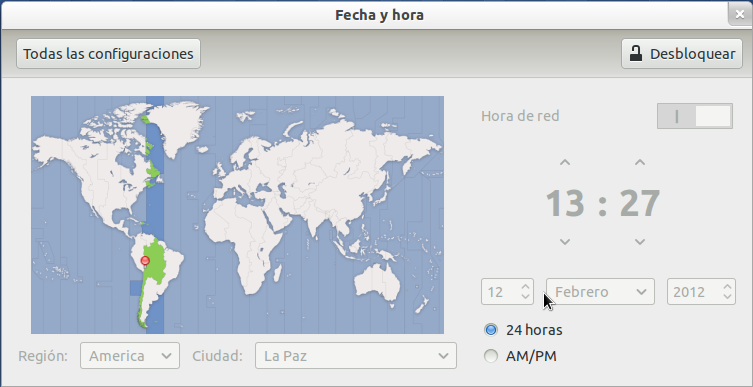
\includegraphics[scale=0.65]{gnome/fechaHora.png} 
		\end{center}
\end{itemize}
\chapter{Configuración de la barra de menú}
\chapter{Acceso a carpetas}
Existen varios gestores de archivos en linux.
Nautilus, es el gestor gráfico de archivos de Gnome, muy fácil de usar.
\begin{itemize}
\item Tiene barra lateral, que se ve muy bien y permite organizar tus “lugares” de forma más sencilla y fácil para navegar por el árbol de directorios.
\item Incorpora una barra de herramientas novedosa e información inteligente de estado.
\item Puede conectarse a un servidor de archivos.
\end{itemize}

\includegraphics[scale=0.6]{gnome-3-nautilus.jpg} 
\chapter{Uso de application launcher}
En este capitulo aprenderemos la forma mas rápida de iniciar aplicaciones\\

Mueva el puntero de su ratón a la esquina de Actividades en la parte superior izquierda de la pantalla para mostrar la Vista de actividades. Aquí es donde puede encontrar todas sus aplicaciones. (También puede abrir la vista pulsando la supertecla o tecla windows.)
Hay distintas maneras de abrir una aplicación una vez que está en la vista de actividades:
\begin{itemize}
\item Comience a escribir las primeras letras de una aplicación; y la búsqueda comenzará al instante. (Si esto no sucede, pulse en la barra de búsqueda en la parte superior derecha de la pantalla y comience a escribir.) Pulse en el icono de la aplicación para iniciarla.
\item Pulse en la cabecera de Aplicaciones en la parte superior de la pantalla para ver una lista de aplicaciones que puede ejecutar. Puede filtrar por tipo, usando las categorías de la derecha, o buscar mediante la barra de búsqueda en la parte superior derecha. Pulse en el icono de la aplicación para iniciarla.
\item Algunas aplicaciones tienen iconos en el tablero, la franja vertical de los iconos en el lado izquierdo de la vista de actividades. Pulse en uno de ellos para iniciar la aplicación correspondiente.\\
Si tiene aplicaciones que usa muy frecuentemente, puede añadirlas al tablero.
\item Puede iniciar una aplicación en un área de trabajo independiente arrastrando el icono de la aplicación desde el tablero (o desde la lista de aplicaciones), y colocándolo en una de las áreas de trabajo en la parte derecha de la pantalla. La aplicación se abrirá en el área de trabajo que elija.
\end{itemize}
Por ejemplo, para lanzar el gestor de archivos, escriba “nautilus” (sin las comillas). El nombre de la aplicación es el comando para lanzar el programa.
\begin{center}
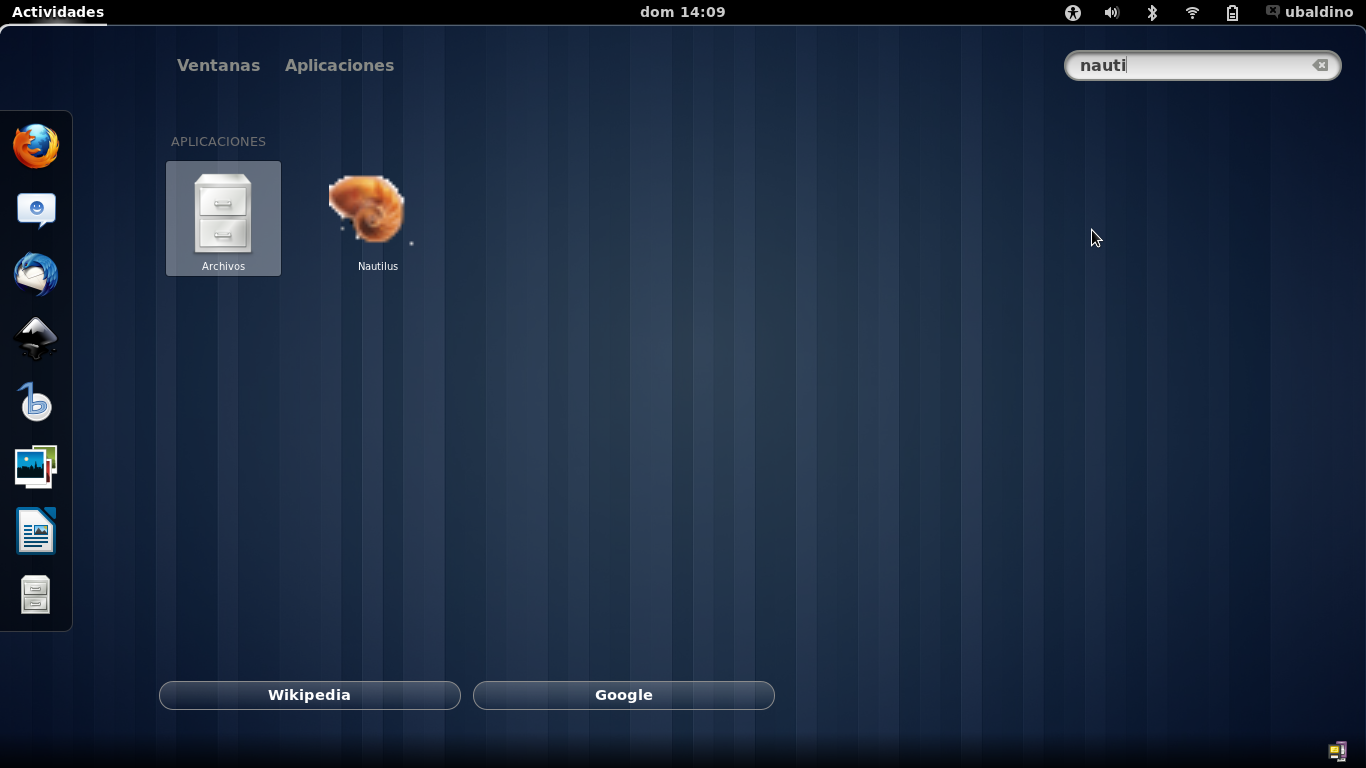
\includegraphics[scale=0.35]{gnome/Pantallazo9.png} 
\end{center}
\end{document}
